% Encoding:UTF-8
% Copyright 2014 MathFire
% Author: Rickjin (ZhihuiJin@gmail.com)
%
\chapter{正态分布的前世今生}
\label{chap:history-of-normal-distribution}

\begin{verse}
\kaishu{
神说,要有正态分布,就有了正态分布。\\
神看正态分布是好的,就让随机误差服从了正态分布。\\
创世纪---数理统计}
\end{verse}

\section{正态分布,熟悉的陌生人}

学过基础统计学的同学大都对正态分布非常熟悉。这个钟形的分布曲线不但形状优雅,它
对应的密度函数写成数学表达式
$$ \displaystyle f(x)=\frac{1}{\sqrt{2\pi}\sigma}e^{-\frac{{(x-\mu})^2}{2\sigma^2}} $$
也非常具有数学的美感。其标准化后的概率密度函数
$$ \displaystyle f(x)=\frac{1}{\sqrt{2\pi}}e^{-\frac{x^2}{2}} $$
更加的简洁漂亮,两个最重要的数学常量 $\pi$、$e$ 都出现在这公式之中。在我个人的
审美之中,它也属于 top-N 的最美丽的数学公式之一,如果有人问我数理统计领域哪个公
式最能让人感觉到上帝的存在,那我一定投正态分布的票。因为这个分布戴着神秘的面纱
,在自然界中无处不在,让你在纷繁芜杂的数据背后看到隐隐的秩序。

\begin{figure}[H]
\centering
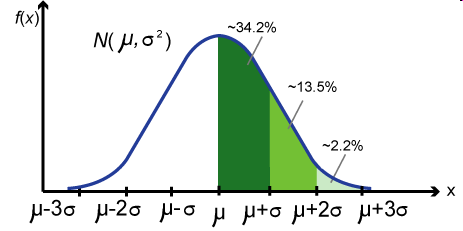
\includegraphics[width=0.8\textwidth]{normal/normal_curve.png}
\caption{正态分布曲线}
\end{figure}

正态分布又通常被称为高斯分布,在科学领域,冠名权那是一个很高的荣誉。2002年以前
去过德国的兄弟们还会发现,德国1991年至2001年间发行的的一款10马克的纸币上印着高
斯(Carl Friedrich Gauss, 1777-1855)的头像和正态密度曲线,而1977年东德发行的20马
克的可流通纪念钢镚上,也印着正态分布曲线和高斯的名字。正态分布被冠名高斯分布,
我们也容易认为是高斯发现了正态分布,其实不然,不过高斯对于正态分布的历史地位的
确立是起到了决定性的作用。

\begin{figure}[htbp]
\centering
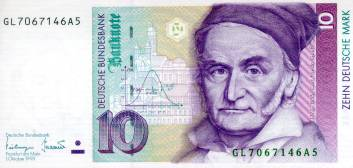
\includegraphics[width=0.8\textwidth]{normal/10dm_with_gauss_curve.jpg}
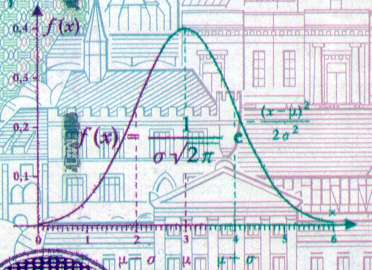
\includegraphics[width=0.4\textwidth]{normal/10dm_with_gauss_curve_detail.jpg}
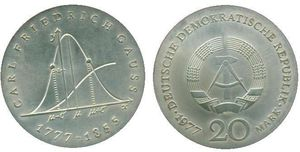
\includegraphics[width=0.4\textwidth]{normal/20-mark-gauss.jpg}
\caption{德国马克和纪念币上的高斯头像和正态分布曲线}
\end{figure}

正态曲线虽然看上去很美,却不是一拍脑袋就能想到的。我们在本科学习数理统计的时候
,课本一上来介绍正态分布就给出分布密度函数,却从来不说明这个密度函数是通过什么
原理推导出来的。所以我一直搞不明白数学家当年是怎么找到这个概率分布曲线的,又是
怎么发现随机误差服从这个奇妙的分布的。我们在实践中大量的使用正态分布,却对这个
分布的来龙去脉知之甚少,正态分布真是让人感觉既熟悉又陌生。直到我读研究生的时候
,我的导师给我介绍了陈希儒院士的《数理统计学简史》这本书,看了之后才了解了正态
分布曲线从发现到被人们重视进而广泛应用,也是经过了几百年的历史。

正态分布的这段历史是很精彩的,我们通过讲一系列的故事来揭开她的神秘面纱。

\section{邂逅,正态曲线的首次发现}

第一个故事和概率论的发展密切相关,主角是棣莫弗(Abraham de Moivre, 1667-1754) 和
拉普拉斯 (Pierre-Simon Laplace 1749-1827)。拉普拉斯是个大科学家,被称为法国的牛
顿;棣莫弗名气可能不算很大,不过大家应该都应该很熟悉这个名字,因为我们在高中数
学学复数的时候都学过棣莫弗公式 $(\cos\theta + i \sin\theta)^n = \cos(n\theta) +
i \sin(n\theta)$。而棣莫弗所写的《机遇论》(The doctrine of chances)是概率论发
展历史中很重要的一本书。牛顿对棣莫弗十分欣赏,遇到学生向他请教概率方面的问题时,
他就说:“这样的问题应该去找棣莫弗,他对这些问题的研究比我深入得多。”

\begin{figure}[htbp]
\centering
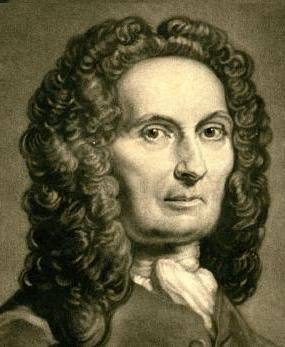
\includegraphics[width=0.25\textwidth]{normal/abraham-de-moivre2.jpg}
\quad \quad
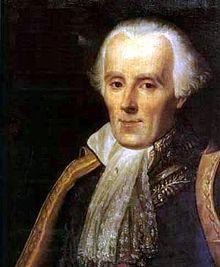
\includegraphics[width=0.25\textwidth]{normal/laplace2.jpg}
\caption{棣莫弗和拉普拉斯}
\end{figure}

古典概率论发源于赌博,惠更斯(Christiaan Huygens, 1629-1695)、帕斯卡(Blaise
Pascal, 1623-1662)、费马(Pierre de Fermat, 1601-1665)、雅可比·贝努利(Jacob
Bernoulli, 1654-1705)都是古典概率的奠基人,他们那会研究的概率问题大都来自赌桌上
,最早的概率论问题是赌徒梅累在1654年向帕斯卡提出的如何分赌金的问题。统计学中的
总体均值之所以被称为期望 (Expectation), 就是源自惠更斯、帕斯卡这些人研究平均情
况下一个赌徒在赌桌上可以期望自己赢得多少钱。

有一天一个哥们,也许是个赌徒,向棣莫弗提了一个和赌博相关的问题:A、B 两人在赌场
里赌博,A、B各自的获胜概率是$p, q=1-p$, 赌 $n$ 局。两人约定:若 A 赢的局数 $X >
np$, 则 A 付给赌场 $X-np$ 元;若 $X<np$,则B 付给赌场 $np-X$ 元。 问赌场挣钱的期
望值是多少。

问题并不复杂, 本质上是一个二项分布,若 $np$ 为整数,棣莫弗求出最后的理论结果是
$$ 2npq b(n, p, np)$$
其中 $ b(n,p,i) = \binom{n}{i}p^iq^{n-i}$ 是常见的二项概率。 但是对具体的 $n$,
因为其中的二项公式中有组合数,要把这个理论结果实际计算出数值结果可不是件容易的
事, 这就驱动棣莫弗寻找近似计算的方法。

与此相关联的另一个问题,是遵从二项分布的随机变量 $ X \sim B(n,p)$, 求X 落在二项
分布中心点一定范围的概率 $ P_d = P(|X - np| \le d)$。

对于 $p=1/2$ 的情形, 棣莫弗做了一些计算并得到了一些近似结果,但是还不够漂亮,
幸运的是棣莫弗和斯特林(James Stirling, 1692-1770)处在同一个时代, 而且二人之间有
联系,斯特林公式是在数学分析中必学的一个重要公式
$$ \displaystyle n! \approx \sqrt{2\pi n} \left(\frac{n}{e}\right)^n .$$

事实上斯特林公式的雏形是棣莫弗最先得到的,但斯特林改进了这个公式,改进的结果为
棣莫弗所用。1733 年,棣莫弗很快利用斯特林公式进行计算并取得了重要的进展。考虑
$n$ 是偶数的情形,二项概率为
$$b(n, \frac{1}{2}, i) = \binom{n}{i}\left(\frac{1}{2}\right)^n$$
以下把$b(n, \frac{1}{2}, i)$简记为$b(i)$, 通过斯特林公式做一些简单的计算容易得到,
$$ \displaystyle b\left(\frac{n}{2}\right) \approx \sqrt{\frac{2}{\pi n}}, $$
$$ \displaystyle \frac{b\left(\frac{n}{2}+d\right)}{b\left(\frac{n}{2}\right)} \approx e^{-\frac{2d^2}{n}}, $$
于是有
$$ \displaystyle b\left(\frac{n}{2}+d\right) \approx \frac{2}{\sqrt{2 \pi n}}e^{-\frac{2d^2}{n}}. $$
使用上式的结果,并在二项概率累加求和的过程中近似的使用定积分代替求和,很容易就
能得到
\begin{eqnarray}
\begin{array}{lll}
\displaystyle P\left(\left|\frac{X}{n} - \frac{1}{2}\right| \le \frac{c}{\sqrt{n}}\right)
& = & \displaystyle \sum_{-c\sqrt{n} \le i \le c\sqrt{n}}b\left(\frac{n}{2}+i\right) \\
& \approx & \displaystyle \sum_{-c\sqrt{n} \le i \le c\sqrt{n}} \frac{2}{\sqrt{2 \pi n}}e^{-\frac{2i^2}{n}}  \\
& = & \displaystyle \sum_{-2c \le \frac{2i}{\sqrt{n}} \le 2c}
\frac{1}{\sqrt{2 \pi}}e^{-\frac{1}{2}(\frac{2i}{\sqrt{n}})^2} \frac{2}{\sqrt{n}} \\
& \approx &\displaystyle  \int_{-2c}^{2c} \frac{1}{\sqrt{2\pi}} e^{-x^2/2} dx .
\end{array}
\end{eqnarray}

看,正态分布的密度函数的形式在积分公式中出现了!这也就是我们在数理统计课本上学
到的一个重要结论:二项分布的极限分布是正态分布。

以上只是讨论了 $p=1/2$ 的情形, 棣莫弗也对 $p \ne 1/2$做了一些计算,后来拉普拉
斯对 $p \ne 1/2$ 的情况做了更多的分析,并把二项分布的正态近似推广到了任意 $p$
的情况。 这是第一次正态密度函数被数学家刻画出来,而且是以二项分布的极限分布的形
式被推导出来的。 熟悉基础概率统计的同学们都知道这个结果其实叫棣莫弗-拉普拉斯中
心极限定理。

\begin{theorem}[棣莫弗-拉普拉斯中心极限定理]
设随机变量 $X_n (n=1,2,\cdots)$ 服从参数为 $n,p$ 的二项分布,则对任意的 $x$, 恒有
$$ \lim_{n\rightarrow\infty}P\left( \frac{X_n - np}{\sqrt{np(1-p)}} \le x \right)
 = \int_{-\infty}^x \frac{1}{\sqrt{2\pi}} e^{\frac{-t^2}{2}}dt .
$$
\end{theorem}

我们在大学学习数理统计的时候,学习的过程都是先学习正态分布,然后才学习中心极限
定理。而学习到正态分布的时候,直接就描述了其概率密度的数学形式,虽然数学上很漂
亮,但是容易困惑数学家们是如何凭空就找到这个分布的。读了陈希孺的《数理统计学简
史》之后,我才明白正态分布的密度形式首次发现是在棣莫弗-拉普拉斯的中心极限定理中
。数学家研究数学问题的进程很少是按照我们数学课本编排的顺序推进的,现代的数学课
本都是按照数学内在的逻辑进行组织编排的,虽然逻辑结构上严谨优美,却把数学问题研
究的历史痕迹抹得一干二净。DNA 双螺旋结构的发现者之一詹姆斯·沃森(James D.
Watson, 1928-) 在他的名著《DNA 双螺旋》序言中说:“ Science seldom proceeds in
the straightforward logical manner imagined by outsiders. (科学的发现很少会像
门外汉所想象的一样,按照直接了当合乎逻辑的方式进行的。)”


棣莫弗给出他的发现后40年(大约是1770年), 拉普拉斯建立了中心极限定理较一般的形
式,中心极限定理随后又被其他数学家们推广到了其它任意分布的情形,而不限于二项分
布。后续的统计学家发现,一系列的重要统计量,在样本量 $N$ 趋于无穷的时候, 其极限
分布都有正态的形式, 这构成了数理统计学中大样本理论的基础。

棣莫弗在二项分布的计算中瞥见了正态曲线的模样,不过他并没有能展现这个曲线的美妙
之处。棣莫弗的这个工作当时并没有引起人们足够的重视,原因在于棣莫弗 不是个统计学
家,从未从统计学的角度去考虑其工作的意义。 正态分布(当时也没有被命名为正态分布)
在当时也只是以极限分布的形式出现,并没有在统计学,尤其是误差分析中发挥作用。这
也就是正态分布最终没有被冠名 棣莫弗分布的重要原因。 那高斯做了啥工作导致统计学
家把正态分布的这顶桂冠戴在了他的头上呢?这先得从最小二乘法的发展说起。

\section{最小二乘法,数据分析的瑞士军刀}

第二个故事的主角是欧拉(Leonhard Euler, 1707-1783)、拉普拉斯、勒让德
(Adrien-Marie Legendre, 1752–1833) 和高斯, 故事发生的时间是18世纪中到19世纪初
。17、18 世纪是科学发展的黄金年代,微积分的发展和牛顿万有引力定律的建立,直接的
推动了天文学和测地学的迅猛发展。当时的大科学家们都在考虑许多天文学上的问题,几
个典型的问题如下:

\begin{enumerate}
\item 土星和木星是太阳系中的大行星,由于相互吸引对各自的运动轨道产生了影响,许
多大数学家,包括欧拉和拉普拉斯都在基于长期积累的天文观测数据计算土星和木星的运
行轨道。

\item 勒让德承担了一个政府给的重要任务,测量通过巴黎的子午线的长度。

\item 海上航行经纬度的定位。主要是通过对恒星和月面上的一些定点的观测来确定经纬度。

\end{enumerate}

这些天文学和测地学的问题,无不涉及到数据的多次测量、分析与计算;17、18世纪的天
文观测,也积累了大量的数据需要进行分析和计算。很多年以前,学者们就已经经验性的
认为,对于有误差的测量数据,多次测量取算术平均是比较好的处理方法。虽然缺乏理论
上的论证,也不断的受到一些人的质疑,取算术平均作为一种异常直观的方式,已经被使
用了千百年, 在多年积累的数据的处理经验中也得到相当程度的验证,被认为是一种良好
的数据处理方法。

以上涉及的问题,我们直接关心的目标量往往无法直接观测,但是一些相关的量是可以观
测到的,而通过建立数学模型,最终可以解出我们关心的量。这些问题都可以用如下数学
模型描述:我们想估计的量是 $\beta_0,\cdots,\beta_p$, 另有若干个可以测量的量
$x_1,\cdots,x_p, y$, 这些量之间有线性关系
$$ y = \beta_0 + \beta_1x_1 + \cdots + \beta_px_p $$
如何通过多组观测数据求解出参数$\beta_0,\cdots,\beta_p$呢? 欧拉和拉普拉斯采用的
的方法都是求解如下线性方程组
\begin{eqnarray}
\left\{
\begin{array}{lll}
 y_1 = \beta_0 + \beta_1x_{11} + \cdots + \beta_px_{p1} \\
 y_2 = \beta_0 + \beta_1x_{12} + \cdots + \beta_px_{p2} \\
\vdots \\
 y_n = \beta_0 + \beta_1x_{1n} + \cdots + \beta_px_{pn} .
\end{array}
\right.
\end{eqnarray}
但是面临的一个问题是,有 $n$ 组观测数据,$p + 1$ 个变量, 如果 $n > p + 1$, 则
得到的线性矛盾方程组,无法直接求解。 所以欧拉和拉普拉斯采用的方法都是通过对数据
的一定的观察,把$n$个线性方程分为 $p+1$组,然后把每个组内的方程线性求和后归并为
一个方程,从而就把$n$个方程的方程组化为$p+1$个方程的方程组,进一步解方程求解
参数。这些方法初看有一些道理,但是都过于经验化, 无法形成统一处理这一类问题的通
用解决框架。

以上求解线性矛盾方程的问题在现在的本科生看来都不困难,这就是统计学中的线性回归
问题,直接用最小二乘法就解决了。可是即便如欧拉、拉普拉斯这些数学大牛,当时也未
能对这些问题提出有效的解决方案。可见在科学研究中,要想在观念上有所突破并不容易
。有效的最小二乘法是勒让德在 1805 年发表的,基本思想就是认为测量中有误差,所以
所有方程的累积误差为
\begin{center}
累积误差 = $\sum($ 观测值 - 理论值 $)^2$
\end{center}
我们求解出导致累积误差最小的参数
\begin{eqnarray}
\label{least-square-error}
\begin{array}{lll}
\hat{\boldsymbol\beta}& = & \displaystyle \argmin_{\boldsymbol {\beta}} \sum_{i=1}^n e_i^2 \\
           & = & \displaystyle
            \argmin_{\boldsymbol\beta} \sum_{i=1}^n\Bigl[y_i - (\beta_0 + \beta_1x_{1i}
            + \cdots + \beta_px_{pi})\Bigr]^2 .
\end{array}
\end{eqnarray}

\begin{figure}[htbp]
\centering
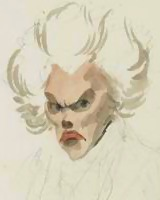
\includegraphics[width=0.3\textwidth]{normal/legendre.jpg}
\caption{勒让德}
\end{figure}

勒让德在论文中对最小二乘法的优良性做了几点说明:
\begin{enumerate}
\item 最小二乘法使得误差平方和最小,并在各个方程的误差之间建立了一种平衡,从而防
      止某一个极端误差取得支配地位;
\item 计算中只要求偏导后求解线性方程组,计算过程明确便捷;
\item 最小二乘法可以导出算术平均值作为估计值。
\end{enumerate}
对于最后一点,推理如下:假设真值为 $\theta$, $x_1, \cdots, x_n$为$n$次测量值, 每
次测量的误差为$ e_i = x_i - \theta $,按最小二乘法,误差累积为
$$ L(\theta) = \sum_{i=1}^n e_i^2 = \sum_{i=1}^n (x_i - \theta)^2 $$
求解$\theta$ 使得 $L(\theta)$达到最小,正好是算术平均 $\overline{x} = \frac{\sum_{i=1}^n x_i}{n} $。

由于算术平均是一个历经考验的方法,而以上的推理说明,算术平均是最小二乘法的一个
特例,所以从另一个角度说明了最小二乘法的优良性,使我们对最小二乘法更加有信心。

最小二乘法发表之后很快得到了大家的认可接受,并迅速的在数据分析实践中被广泛使用
。不过历史上又有人把最小二乘法的发明归功于高斯,这又是怎么一回事呢。高斯在1809
年也发表了最小二乘法,并且声称自己已经使用这个方法多年。高斯发明了小行星定位的
数学方法,并在数据分析中使用最小二乘法进行计算,准确的预测了谷神星的位置。

扯了半天最小二乘法,没看出和正态分布有任何关系啊,离题了吧?单就最小二乘法本身
,虽然很实用,不过看上去更多的算是一个代数方法,虽然可以推导出最优解,对于解的
误差有多大,无法给出有效的分析,而这个就是正态分布粉墨登场发挥作用的地方。勒让
德提出的最小二乘法,确实是一把在数据分析领域披荆斩棘的好刀,但是刀刃还是不够锋
利;而这把刀的打造后来至少一半功劳被归到高斯,是因为高斯不但独自的给出了造刀的
方法,而且把最小二乘这把刀的刀刃磨得无比锋利,把最小二乘法打造成了一把瑞士军刀。
高斯拓展了最小二乘法,把正态分布和最小二乘法联系在一起,并使得正态分布在统计误
差分析中确立了自己的地位,否则正态分布就不会被称为高斯分布了。 那高斯这位神人是
如何把正态分布引入到误差分析之中,打造最小二乘法这把瑞士军刀的呢?

\section{众里寻她千百度,误差分布曲线的确立}

第三个故事有点长,主角是高斯和拉普拉斯,故事的主要内容是寻找随机误差分布的规律。

天文学是第一个被测量误差困扰的学科,从古代至18世纪天文学一直是应用数学最发达的
领域,到18世纪,天文学的发展积累了大量的天文学数据需要分析计算,应该如何来处理
数据中的观测误差成为一个很棘手的问题。我们在数据处理中经常使用平均的常识性法则
,千百来来的数据使用经验说明算术平均能够消除误差,提高精度。算术平均有如此的魅
力,道理何在,之前没有人做过理论上的证明。算术平均的合理性问题在天文学的数据分
析工作中被提出来讨论:测量中的随机误差应该服从怎样的概率分布?算术平均的优良性
和误差的分布有怎样的密切联系?

伽利略在他著名的《关于两个主要世界系统的对话》中,对误差的分布做过一些定性的描
述,主要包括:
\begin{enumerate}
\item 观测数据存在误差
\item 误差是对称分布的;
\item 大的误差出现频率低,小的误差出现频率高。
\end{enumerate}
用数学的语言描述,也就是说误差分布的密度函数 $f(x)$ 关于0对称分布,概率密度随
$|x|$ 增加而减小,这两个定性的描述都很符合常识。

许多天文学家和数学家开始了寻找误差分布曲线的尝试。 天文学家辛普森(Thomas
Simpson, 1710-1761) 先走出了有意义的一步。设真值为 $\theta$, $x_1, \cdots, x_n$
为n次测量值, 每次测量的误差为$ e_i = x_i - \theta $,若用算术平均 $\overline{x} =
\frac{\sum_{i=1}^n x_i}{n} $去估计$\theta$, 其误差为 $\overline{e} =
\frac{\sum_{i=1}^n e_i}{n} $。 辛普森证明了, 对于如下的一个概率分布,

\begin{figure}[ht]
\centering
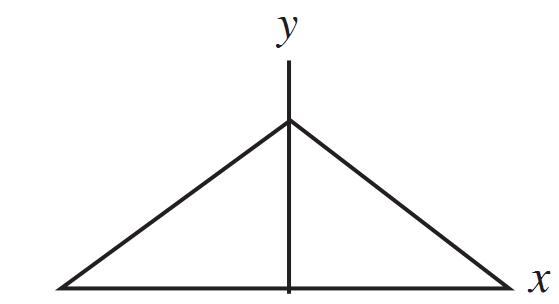
\includegraphics[width=0.8\textwidth]{normal/simpson-error-curve.jpg}
\caption{辛普森的误差分布曲线}
\end{figure}

有如下结论
$$P(|\overline{e}| < x) \ge P(|e_i|<x) . $$
也就是说,$|\overline{e}|$ 相比于$|e_i|$取小值的机会更大。 辛普森的这个工作很粗糙
,但是这是第一次在一个特定情况下,从概率论的角度严格证明了算术平均的优良性。

从 1772-1774 年, 拉普拉斯也加入到了寻找误差分布密度函数的队伍中。拉普拉斯假定误差
分布密度函数$f(x)$对称且满足
$$ -f'(x) = mf(x) $$
由此可求得分布密度函数为
\begin{equation}
\label{laplace-error-curve}
f(x) = \frac{m}{2} e^{-m|x|} .
\end{equation}
这个概率密度函数现在被称为拉普拉斯分布。

\begin{figure}[ht]
\centering
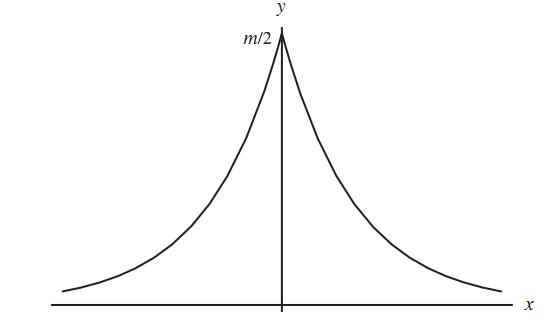
\includegraphics[width=0.8\textwidth]{normal/laplace-error-curve.jpg}
\caption{拉普拉斯的误差分布曲线}
\end{figure}


以(\ref{laplace-error-curve})式中的函数作为误差分布,拉普拉斯开始考虑如何基于测
量的结果去估计未知参数的值。拉普拉斯可以算是一个贝叶斯主义者,他的参数估计的原
则和现代贝叶斯方法非常相似:假设先验分布是均匀的,计算出参数的后验分布后,取后
验分布的中值点,即$1/2$分位点,作为参数估计值。可是基于这个误差分布密度函数做了
一些计算之后,拉普拉斯发现计算过于复杂,最终没能给出什么有用的结果。

拉普拉斯可是概率论的大牛,写过在概率发展历史中极有影响力的《分析概率论》,不过以我的数学审
美,实在无法理解拉普拉斯这样的牛人怎么找了一个零点不可导的函数作为误差的分布密
度函数,拉普拉斯最终还是没能搞定误差分布的问题。

现在轮到高斯登场了,高斯在数学史中的地位极高,年轻的时候号称数学王子,后来被称
为数学家中的老狐狸,数学家阿贝尔 (Niels Henrik Abel, 1802-1829) 对他的评论是 :
“高斯像一只狐狸,用尾巴将沙地上的足迹抹去(He is like the fox, who effaces his
tracks in the sand with his tail) 。” 我们的数学大师陈省身把黎曼(Georg
Friedrich Bernhard Riemann,1826-1866) 和庞加莱(Jules Henri Poincar\'{e},
1854-1912)称为数学家中的菩萨,而称自己为罗汉;高斯是黎曼的导师,数学圈里有些教
授把高斯称为数学家中的佛。 在数学家中既能仰望理论数学的星空,又能脚踏应用数学的
实地的可不多见,高斯是数学家中少有的顶”天“立”地“的人物,它既对纯理论数学有
深刻的洞察力,又极其重视数学在实践中的应用。 在误差分布的处理中,高斯以极其简单
的手法确立了随机误差的概率分布,其结果成为数理统计发展史上的一块里程碑。

高斯的介入首先要从天文学界的一个事件说起。1801年1月,天文学家朱塞普·皮亚齐
(Giuseppe Piazzi, 1746-1826)发现了一颗从未见过的光度8等的星在移动,这颗现在被称
作谷神星(Ceres)的小行星在夜空中出现6个星期,扫过八度角后就在太阳的光芒下没了
踪影,无法观测。而留下的观测数据有限,难以计算出他的轨道,天文学家也因此无法确
定这颗新星是彗星还是行星,这个问题很快成了学术界关注的焦点。高斯当时已经是很有
名望的年轻数学家了,这个问题引起了他的兴趣。高斯以其卓越的数学才能创立了一种崭
新的行星轨道的计算方法,一个小时之内就计算出了谷神星的轨道,并预言了他在夜空中
出现的时间和位置。 1801年12月31 日夜,德国天文爱好者奥伯斯(Heinrich Olbers,
1758-1840),在高斯预言的时间里,用望远镜对准了这片天空。果然不出所料,谷神星出
现了!

高斯为此名声大震,但是高斯当时拒绝透露计算轨道的方法,原因可能是高斯认为自己的
方法的理论基础还不够成熟,而高斯一向治学严谨、精益求精,不轻易发表没有思考成熟
的理论。直到1809年高斯系统地完善了相关的数学理论后,才将他的方法公布于众,而其
中使用的数据分析方法,就是以正态误差分布为基础的最小二乘法。那高斯是如何推导出
误差分布为正态分布的?让我们看看高斯是如何猜测上帝的意图的。

设真值为 $\theta$, $x_1, \cdots, x_n$为$n$次独立测量值, 每次测量的误差为$ e_i = x_i - \theta $,
假设误差$e_i$的密度函数为 $f(e)$, 则测量值的联合概率为$n$个误差的联合概率,记为
\begin{align*}
L(\theta) & = L(\theta;x_1,\cdots,x_n)=f(e_1)\cdots f(e_n) \\
& = f(x_1-\theta)\cdots f(x_n-\theta)
\end{align*}
但是高斯不采用贝叶斯的推理方式,而是直接取使$L(\theta)$达到最大值的
$\hat{\theta}=\hat{\theta}(x_1,\cdots,x_n)$ 作为$\theta$的估计值,即
$$ \hat{\theta}= \argmax_{\theta} L(\theta) .$$
现在我们把$L(\theta)$ 称为样本的似然函数,而得到的估计值$ \hat{\theta}$ 称为极
大似然估计。高斯首次给出了极大似然的思想,这个思想后来被统计学家费希尔系统的发
展成为参数估计中的极大似然估计理论。

数学家波利亚(George P\'{o}lya, 1887-1985)说过:“要成为一个好的数学家,……,你必须
首先是一个好的猜想家(To be a good mathematician,..., you must be a good
guesser)。”历史上一流的数学家都是伟大的猜想家。高斯接下来的想法特别牛,他开始
揣度上帝的意图,而这充分体现了高斯的数学天才。高斯把整个问题的思考模式倒过来:
既然千百年来大家都认为算术平均是一个好的估计,那我就认为极大似然估计导出的就应
该是算术平均!所以高斯猜测上帝在创世纪中的旨意就是:
\begin{center}
\bf{误差分布导出的极大似然估计 = 算术平均值}
\end{center}

然后高斯去找误差密度函数 $f$ 以迎合这一点。即寻找这样的概率分布密度函数 $f$, 使
得极大似然估计正好是算术平均 $\hat{\theta} = \overline{x}$。而高斯应用数学技巧求解这
个函数$f$, 高斯证明(证明不难,后续给出),所有的概率密度函数中,唯一满足这个性质
的就是 $$ \displaystyle
f(x)=\frac{1}{\sqrt{2\pi}\sigma}e^{-\frac{x^2}{2\sigma^2}} $$ 瞧,正态分布的密
度函数 $N(0, \sigma^2)$ 被高斯他老人家给解出来了!

进一步,高斯基于这个误差分布的密度函数对最小二乘法给出了一个很漂亮的解释。对于
最小二乘公式中涉及的每个误差 $e_i$(见上文公式(\ref{least-square-error})), 由于
误差服从概率分布 $N(0, \sigma^2)$, 则$(e_1, \cdots, e_n)$ 的概率为
$$\frac{1}{(\sqrt{2\pi}\sigma)^n}\exp\left\{-\frac{1}{2\sigma^2} \sum_{i=1}^n e_i^2 \right\} .$$
要使得这个概率最大,必须使得$\sum_{i=1}^n e_i^2 $ 取最小值,这正好就是最小二
乘法的要求。

高斯所拓展的最小二乘法成为了19世纪统计学的最重要成就,它在19世纪统计学的重要性
就相当于18世纪的微积分之于数学。而勒让德和高斯的关于最小二乘法的发明权之争,成
了数学史上仅次于牛顿、莱布尼茨微积分发明权的争端。相比于勒让德1805年给出的最小
二乘法描述,高斯基于误差正态分布的最小二乘理论显然更高一筹,高斯的工作中既提出
了极大似然估计的思想,又解决了误差的概率密度分布的问题,由此我们可以对误差大小
的影响进行统计度量了。高斯的这项工作对后世的影响极大,而正态分布也因此被冠名高
斯分布。估计高斯本人当时是完全没有意识到他的这个工作给现代数理统计学带来的深刻
影响。高斯在数学上的贡献特多,去世前他是要求给自己的墓碑上雕刻上正十七边形,以
说明他在正十七边形尺规作图上的杰出工作。而后世的德国钞票和钢镚上是以正态密度曲
线来纪念高斯,这足以说明高斯的这项工作在当代科学发展中的分量。

17、18世纪科学界流行的做法,是尽可能从某种简单明了的准则(first principle)出
发进行逻辑推导。高斯设定了准则“最大似然估计应该导出优良的算术平均”,并导出了
误差服从正态分布,推导的形式上非常简洁优美。但是高斯给的准则在逻辑上并不足以让
人完全信服,因为算术平均的优良性当时更多的是一个经验直觉,缺乏严格的理论支持。
高斯的推导存在循环论证的味道:因为算术平均是优良的,推出误差必须服从正态分布;
反过来,又基于正态分布推导出最小二乘法和算术平均,来说明最小二乘法和算术平均的优
良性。这陷入了一个鸡生蛋蛋生鸡的怪圈,逻辑上算术平均的优良性到底有没有自行成立
的理由呢?

高斯的文章发表之后,拉普拉斯很快得知了高斯的工作。拉普拉斯看到,正态分布既可以
从抛钢镚产生的序列和中生成出来,又可以被优雅的作为误差分布定律,这难道是偶然现
象?拉普拉斯不愧为概率论的大牛,他马上将误差的正态分布理论和中心极限定理联系起
来,提出了元误差解释。他指出如果误差可以看成许多微小量的叠加,则根据他的中心极
限定理,随机误差理所应当是高斯分布。而20世纪中心极限定理的进一步发展,也给这个
解释提供了更多的理论支持。因此以这个解释为出发点,高斯的循环论证的圈子就可以
打破。 估计拉普拉斯悟出这个结论之后一定想撞墙,自己辛辛苦苦寻寻觅觅了这么久的误
差分布曲线就在自己的眼皮底下,自己却长年视而不见,被高斯占了先机。

至此,误差分布曲线的寻找尘埃落定,正态分布在误差分析中确立了自己的地位,并在整
个19世纪不断的开疆扩土,直至在统计学中鹤立鸡群,傲世其它一切概率分布;而高斯和
拉普拉斯的工作,为现代统计学的发展开启了一扇大门。

在整个正态分布被发现与应用的历史中,棣莫弗、拉普拉斯、高斯各有贡献,拉普拉斯从
中心极限定理的角度解释它,高斯把它应用在误差分析中,殊途同归。正态分布被人们发
现有这么好的性质,各国人民都争抢它的冠名权。因为拉普拉斯是法国人,所以当时在法
国被称为拉普拉斯分布;而高斯是德国人, 所以在德国叫做高斯分布;第三中立国的人民
称他为拉普拉斯-高斯分布。后来法国的大数学家庞加莱建议改用正态分布这一中立名称,
而随后统计学家卡尔·皮尔森使得这个名称被广泛接受:

\begin{quotation}
\emph{Many years ago I called the Laplace-Gaussian curve the normal curve,
which name, while it avoids an international question of priority,
has the disadvantage of leading people to believe that all other distributions
of frequency are in one sense or another "abnormal".}

\emph{ ---Karl Pearson (1920) }
\end{quotation}

不过因为高斯在数学家中的名气实在是太大, 正态分布的桂冠还是更多地被戴在了高斯的脑
门上,目前数学界通行的用语是正态分布、高斯分布, 两者并用。

正态分布在高斯的推动下,迅速在测量误差分析中被广泛使用,然而早期也仅限于测量误
差的分析中,其重要性远没有被自然科学和社会科学领域中的学者们所认识,那正态分布
是如何从测量误差分析的小溪,冲向自然科学和社会科学的汪洋大海的呢?

\section{曲径通幽处,禅房花木深}

在介绍正态分布的后续发展之前,我们来多讲一点数学,也许有些人会觉得枯燥,不过高
斯曾经说过:“数学是上帝的语言”;所以要想更加深入的理解正态分布的美,唯有借助
于上帝的语言。

造物主造物的准则往往是简单明了的,只是在纷繁芜杂的万物之中,我们要发现并领会它
并非易事。之前提到过,17、18世纪科学界流行的做法,是尽可能从某种简单明了的准则
出发作为科学探求的起点;而后来的数学家和物理学家们的研究发现,屡次从一些给定的
简单的准则出发, 我们总是被引领到了正态分布的家门口,这让人感觉到正态分布的美妙。

达尔文的表弟高尔顿是生物学家兼统计学家,他对正态分布非常的推崇与赞美:”我几乎
不曾见过像误差呈正态分布这么激发人们无穷想象的宇宙秩序“。当代两位伟大的概率学
家列维(Paul Pierre L\'{e}vy, 1886-1971) 和卡克(Mark Kac, 1914-1984) 都曾经说过,
正态分布是他们切入概率论的初恋情人,具有无穷的魅力。如果古希腊人知道正态分布,
想必奥林匹斯山的神殿里会多出一个正态女神,由她来掌管世间的混沌。

要拉下正态分布的神秘面纱展现她的美丽,需要高深的概率论知识,本人在数学方面知识
浅薄,不能胜任。只能在极为有限的范围内尝试掀开她的面纱的一角。棣莫弗和拉普拉斯
以抛钢镚的序列求和为出发点,沿着一条小径第一次把我们领到了正态分布的家门口,这
条路叫做中心极限定理。而这条路上风景秀丽,许多概率学家都为之倾倒。这条路在二十
世纪被概率学家们越拓越宽,成为了通往正态曲线的一条康庄大道。而数学家和物理学家
们发现:条条小路通正态。著名的物理学家杰恩斯(Edwin Thompson Jaynes, 1922-1998)
在他的名著《概率论沉思录(Probability Theory: the Logic of Science)》中,描绘了
四条通往正态分布的小径;曲径通幽处,禅房花木深,让我们一起来欣赏一下这四条小径
上的风景吧。

\subsection{高斯(1809)的推导}

第一条小径是高斯找到的,高斯以如下准则作为小径的出发点
\begin{center}
误差分布导出的极大似然估计 = 算术平均值
\end{center}

设真值为 $\theta$, $x_1, \cdots, x_n$为n次独立测量值, 每次测量的误差为$ e_i =
x_i - \theta $,假设误差$e_i$的密度函数为 $f(e)$, 则测量值的联合概率为$n$个误差的联
合概率,记为
\begin{align*}
L(\theta) &= L(\theta;x_1,\cdots,x_n)=f(e_1)\cdots f(e_n)  \\
& = f(x_1-\theta)\cdots f(x_n-\theta)
\end{align*}
为求极大似然估计,令
$$\frac{d \log L(\theta)}{d \theta} = 0$$
整理后可以得到
$$ \sum_{i=1}^n \frac{f'(x_i-\theta)}{f(x_i-\theta)} = 0 $$
令 $g(x) = \frac{f'(x)}{f(x)}$,
$$ \sum_{i=1}^n g(x_i-\theta) = 0 $$
由于高斯假设极大似然估计的解就是算术平均 $\bar{x}$,把解代入上式,可以得到
\begin{equation}
\label{gauss-derivation}
\sum_{i=1}^n g(x_i-\bar{x}) = 0
\end{equation}
(\ref{gauss-derivation})式中取 $n=2$, 有
$$g(x_1-\bar{x}) + g(x_2-\bar{x}) = 0$$
由于此时有 $ x_1-\bar{x} = -(x_2-\bar{x})$, 并且 $x_1, x_2$ 是任意的,由此得到
$$ g(-x) = -g(x) $$
(\ref{gauss-derivation})式中再取 $n=m+1$, 并且要求 $x_1=\cdots=x_m=-x, x_{m+1} =
mx$, 则有 $\bar{x} = 0$, 并且
$$ \sum_{i=1}^n g(x_i-\bar{x}) = mg(-x) + g(mx) $$
所以得到
$$g(mx) = mg(x)$$
而满足上式的唯一的连续函数就是 $g(x)=cx$, 从而进一步可以求解出
$$f(x) = Me^{cx^2}$$
由于$f(x)$是概率密度函数,把$f(x)$ 正规化一下就得到均值为$0$的正态分布密度函数
$N(0,\sigma^2)$。

\subsection{赫歇尔(1850)和麦克斯韦(1860) 的推导}

第二条小径是天文学家赫歇尔(John Frederick William Herschel, 1792-1871)和物理学
家麦克斯韦(James Clerk Maxwell, 1831-1879) 发现的。 1850年,天文学家赫歇尔在对星
星的位置进行测量的时候,需要考虑二维的误差分布,为了推导这个误差的概率密度分布
$p(x,y)$,赫歇尔设置了两个准则:
\begin{enumerate}
\item $x$ 轴和 $y$ 轴的误差是相互独立的,即随机误差在正交的方向上相互独立
\item 误差的概率分布在空间上具有旋转对称性,即误差的概率分布和角度没有关系
\end{enumerate}
这两个准则对于赫歇尔考虑的实际测量问题看起来都很合理。由第一条准则,可以得到
$p(x,y)$ 应该具有如下形式
$$ p(x,y) = f(x) * f(y) $$
把这个函数转换为极坐标,在极坐标下的概率密度函数设为 $g(r,\theta)$, 有
$$ p(x,y) =  p(rcos\theta, rsin\theta) = g(r,\theta)$$
由第二条准则, $g(r,\theta)$ 具有旋转对称性,也就是应该和 $\theta$ 无关, 所以 $g(r,\theta)=g(r)$,
综上所述,我们可以得到
$$ f(x)f(y) = g(r) = g(\sqrt{x^2+y^2}) $$
取 $y=0$, 得到 $g(x) = f(x)f(0)$, 所以上式可以转换为
$$ \log\left[\frac{f(x)}{f(0)}\right] + \log\left[\frac{f(y)}{f(0)}\right]
= \log\left[\frac{f(\sqrt{x^2+y^2})}{f(0)}\right] $$
令 $\log\left[\frac{f(x)}{f(0)}\right] = h(x) $, 则有
$$ h(x) + h(y) = h(\sqrt{x^2+y^2}) $$
从这个函数方程中可以解出 $h(x) = ax^2$, 从而可以得到 $f(x)$ 的一般形式如下
$$ f(x) = \sqrt{\frac{\alpha}{\pi}} e^{-\alpha x^2} $$
而 $f(x)$ 就是正态分布 $N(0, 1/\sqrt{2\alpha)}$, 从而 $p(x,y)$ 就是标准二维正态
分布的密度函数
$$ p(x,y) = \frac{\alpha}{\pi} e^{-\alpha (x^2+y^2)}. $$

1860 年,伟大的物理学家麦克斯韦在考虑气体分子的运动速度分布的时候,在三维空
间中基于类似的准则推导出了气体分子运动的分布是正态分布
$\rho(v_x,v_y,v_z) \propto \exp\{-\alpha(v_x^2+v_y^2+v_z^2)\} $。这就是著名的麦
克斯韦分子速率分布定律。大家还记得我们在普通物理中学过的麦克斯韦-波尔兹曼气体速
率分布定律吗?
\begin{eqnarray}
\label{maxwell}
\begin{array}{lll}
F(v) & = & \displaystyle \left(\frac{m}{2\pi kT}\right)^{3/2} e^{-\frac{mv^2}{2kT}} \\
& = & \displaystyle  \left(\frac{m}{2\pi kT}\right)^{1/2} e^{-\frac{mv_x^2}{2kT}}
                     \times \left(\frac{m}{2\pi kT}\right)^{1/2} e^{-\frac{mv_y^2}{2kT}}
                     \times \left(\frac{m}{2\pi kT}\right)^{1/2} e^{-\frac{mv_z^2}{2kT}} .
\end{array}
\end{eqnarray}
所以这个分布其实是三个正态分布的乘积, 你的物理老师是否告诉过你其实这个分布就是
三维正态分布?

赫歇尔-麦克斯韦推导的神妙之处在于,没有利用任何概率论的知识,只是基于空间几何的
不变性,就推导出了正态分布。美国诺贝尔奖物理学家费曼(Richard Feymann,1918-1988)
每次看到一个有 $\pi$的数学公式的时候,就会问:圆在哪里?这个推导中使用到了
$x^2+y^2$, 也就是告诉我们正态分布密度公式中有个$\pi$, 其根源在于二维正态分布中
的等高线恰好是个圆。

\subsection{兰登(1941)的推导}

第三条道是一位电气工程师兰登(Vernon D. Landon)给出的。1941 年, 兰登研究通信电
路中的噪声电压,通过分析经验数据他发现噪声电压的分布模式很相似,不同的是分布的
层级,而这个层级可以使用方差 $\sigma^2$ 来刻画。因此他推理认为噪声电压的分布密度函
数形式是 $p(x;\sigma^2)$。假设原来的电压为X, 累加了一个相对其方差 $\sigma$而言
很微小的误差扰动 $\epsilon$, $\epsilon$ 的概率密度是 $q(e)$, 那么新的噪声电压
是 $X' = X + \epsilon$。 兰登提出了如下的准则

\begin{enumerate}
\item 随机噪声具有稳定的分布模式
\item 累加一个微小的随机噪声,不改变其稳定的分布模式,只改变分布的层级(用方差度量)
\end{enumerate}
用数学的语言描述: 如果 $$X \sim p(x;\sigma^2), \epsilon \sim q(e), X'= X+\epsilon$$
则有 $$X' \sim p(x;\sigma^2 + var(\epsilon))$$

现在我们来推导函数$p(x;\sigma^2)$ 应该长成啥样。按照两个随机变量和的分布的计算
方式, $X'$ 的分布密度函数将是 $X$ 的分布密度函数和 $\epsilon$的分布密度函数的
卷积,即有
$$ f(x') = \int p(x'-e; \sigma^2)q(e)de $$
把 $p(x'-e; \sigma^2)$ 在$x'$处做泰勒级数展开(为了方便,展开后把自变量由 $x'$
替换为 $x$), 上式可以展开为
$$ f(x) = p(x; \sigma^2) - \frac{\partial p(x; \sigma^2)}{\partial x} \int eq(e)de +
\frac{1}{2} \frac{\partial^2 p(x; \sigma^2)}{\partial x^2} \int e^2q(e)de + \cdots
$$
将$p(x; \sigma^2)$简记为$p$,则有
$$ f(x) = p - \frac{\partial p}{\partial x} \overline{\epsilon} +
\frac{1}{2} \frac{\partial^2 p}{\partial x^2}\overline{\epsilon^2} + o(\overline{\epsilon^2})
$$

对于微小的随机扰动 $\epsilon$, 我们认为他取正值或者负值是对称的,所以
$\overline{\epsilon} = 0 $。所以有
\begin{equation}
\label{landon-x}
 f(x) = p + \frac{1}{2} \frac{\partial^2 p}{\partial x^2}\overline{\epsilon^2} + o(\overline{\epsilon^2})
\end{equation}

对于新的噪声电压 $X' = X + \epsilon$, 方差由$\sigma^2$ 增加为 $\sigma^2 + var(\epsilon) =
\sigma^2 + \overline{\epsilon^2}$,所以按照兰登的分布密度函数模式不变的假设, 新的
噪声电压的分布密度函数应该为 $f(x) = p(x; \sigma^2 +  \overline{\epsilon^2})$。把$p(x;
\sigma^2 +  \overline{\epsilon^2})$ 在 $\sigma^2$ 处做泰勒级数展开,得到
\begin{equation}
\label{landon-sigma}
f(x) = p + \frac{\partial p}{\partial \sigma^2}\overline{\epsilon^2} + o(\overline{\epsilon^2})
\end{equation}
比较 (\ref{landon-x}) 和 (\ref{landon-sigma}) 这两个式子,可以得到如下偏微分方程
$$ \frac{1}{2} \frac{\partial^2 p}{\partial x^2} = \frac{\partial p}{\partial \sigma^2} $$
而这个方程就是物理上著名的扩散方程(diffusion equation),求解该方程就得到
$$ p(x; \sigma^2) = \frac{1}{\sqrt{2\pi}\sigma}e^{-\frac{x^2}{2\sigma^2}} $$
又一次,我们推导出了正态分布!

杰恩斯对于这个推导的评价很高,认为兰登 的推导本质上给出了自然界的噪音形
成过程。他指出这个推导这基本上就是中心极限定理的增量式版本,相比于中心极限定
理是一次性累加所有的因素,兰登 的推导是每次在原有的分布上去累加一个微小的扰动
。而在这个推导中,我们看到,正态分布具有相当好的稳定性;只要数据中正态的模式已
经形成,他就容易继续保持正态分布,无论外部累加的随机噪声 $q(e)$ 是什么分布,正
态分布就像一个黑洞一样把这个累加噪声吃掉。

\subsection{基于最大熵的推导}

还有一条小径是基于最大熵原理的, 物理学家杰恩斯在最大熵原理上有非常重要的
贡献,他在《概率论沉思录》里面对这个方法有描述和证明,没有提到发现者,我不确认
这条道的发现者是否是杰恩斯本人。

熵在物理学中由来已久,信息论的创始人香农(Claude Elwood Shannon, 1916-2001)把这个
概念引入了信息论,学习机器学习的同学们都知道目前机器学习中有一个非常好用的分类
算法叫最大熵分类器。要想把熵和最大熵的来龙去脉说清楚可不容易,不过这条道的风景
是相当独特的,杰恩斯对这条道也是偏爱有加。

对于一个概率分布 $p(x)$, 我们定义他的熵为
$$H(p) = -\int p(x)\log p(x) dx$$

如果给定一个分布密度函数 $p(x)$ 的均值 $\mu$ 和方差 $\sigma^2$(给定均值和方差这个条
件,也可以描述为给定一阶原点矩和二阶原点矩,这两个条件是等价的), 则在所有满足
这两个限制的概率分布中,熵最大的概率分布 $p(x|\mu, \sigma^2)$ 就是正态分布
$N(\mu, \sigma^2)$。

这个结论的推导数学上稍微有点复杂,不过如果已经猜到了给定限制条件下最大熵的分布
是正态分布,要证明这个猜测却是很简单的,证明的思路如下。

考虑两个概率分布 $p(x)$和$q(x)$,使用不等式 $\log x \le (x-1) $, 得
$$ \int p(x) \log \frac{q(x)}{p(x)} dx \le \int p(x) (\frac{q(x)}{p(x)} - 1) dx
= \int q(x) dx - \int p(x) dx = 0 $$
于是
$$ \int p(x) \log \frac{q(x)}{p(x)} dx = \int p(x) \log\frac{1}{p(x)}dx + \int p(x) \log q(x) dx \le 0 $$
所以
\begin{equation}
 H(p) \le -\int p(x) \log q(x) dx
\end{equation}
熟悉信息论的同学都知道,这个式子是信息论中的很著名的结论:一个概率分布的熵总是
小于交叉熵。上式要取等号当且仅当$q(x)=p(x)$。

对于 $p(x)$, 在给定的均值 $\mu$ 和方差 $\sigma^2$下, 我们取$q(x)=N(\mu,
\sigma^2)$, 则可以得到
\begin{eqnarray}
\begin{array}{lll}
 H(p) &  \le &\displaystyle - \int p(x) \log \left\{ \frac{1}{\sqrt{2\pi}\sigma}
 e^{-\frac{{(x-\mu})^2}{2\sigma^2}}\right\} dx \\
 & = & \displaystyle \int p(x) \left\{ \frac{(x-\mu)^2}{2\sigma^2}  + \log \sqrt{2\pi}\sigma \right\} dx \\
 & = & \displaystyle \frac{1}{2\sigma^2} \int p(x)(x-\mu)^2 dx + \log \sqrt{2\pi}\sigma
\end{array}
\end{eqnarray}
由于 $p(x)$ 的均值方差有如下限制
$$ \int p(x) (x-\mu)^2 dx = \sigma^2$$
于是
$$  H(p) \le \frac{1}{2\sigma^2}\sigma^2 + \log \sqrt{2\pi}\sigma  =  \frac{1}{2} + \log \sqrt{2\pi}\sigma $$
而当$p(x)=N(\mu, \sigma^2)$的时候,上式可以取到等号,这就证明了结论。


杰恩斯显然对正态分布具有这样的性质极为赞赏,因为这从信息论的角度证明了正态
分布的优良性。而我们可以看到,正态分布熵的大小,取决于方差的大小。 这也容易理解
, 因为正态分布的均值和密度函数的形状无关,正态分布的形状是由其方差决定的,而熵
的大小反应概率分布中的信息量,显然和密度函数的形状相关。

好的,风景欣赏暂时告一段落。所谓“横看成岭侧成峰,远近高低各不同”,正态分布给
人们提供了多种欣赏角度和想象空间。法国菩萨级别的大数学家庞加莱对正态分布说过一
段有意思的话,引用来作为这个小节的结束:
\begin{quotation}
\emph{
Physicists believe that the Gaussian law has been proved in mathematics
while mathematicians think that it was experimentally established in physics. }
\kaishu{(物理学家认为高斯分布已经在数学上得到证明,而数学家则认为高斯分布在物理试验中得
到确认。) }
\\
\emph{--- Henri Poincar\'{e}}
\end{quotation}

\section{开疆拓土,正态分布的进一步发展}

19世纪初,随着拉普拉斯中心极限定理的建立与高斯正态误差理论的问世,正态分布开始
崭露头角,逐步在近代概率论和数理统计学中大放异彩。在概率论中,由于拉普拉斯的推
动,中心极限定理发展成为现代概率论的一块基石;而在数理统计学中,在高斯的大力提
倡之下,正态分布开始逐步畅行于天下。

\subsection{论剑中心极限定理}

先来说说正态分布在概率论中的地位,这个主要是由于中心极限定理的影响。 1776 年,
拉普拉斯开始考虑一个天文学中的彗星轨道的倾角的计算问题,最终的问题涉及独立随机
变量求和的概率计算,也就是计算如下的概率值
$$ S_n = X_1 + X_2 + \cdots + X_n  $$
$$P(a < S_n < b) = ? $$

在这个问题的处理上,拉普拉斯充分展示了其深厚的数学分析功底和高超的概率计算技巧
,他首次引入了特征函数(也就是对概率密度函数做傅立叶变换)来处理概率分布的神妙方
法,而这一方法经过几代概率学家的发展,在现代概率论里面占有极其重要的位置。基于
这一分析方法,拉普拉斯通过近似计算,在他1812年发表的名著《分析概率论》中给
出了中心极限定理的一般描述:

\begin{theorem}[拉普拉斯, 1812] $ e_i (i=1, \cdots n)$ 为独立同分布的测量误差,
具有均值$\mu$ 和方差 $\sigma^2$,如果 $\lambda_1, \cdots, \lambda_2$ 为常数,
$a>0$, 则有
$$ \displaystyle P\left(\left|\sum_{i=1}^n \lambda_i(e_i - \mu)\right|
\le a \sqrt{\sum_{i=1}^n \lambda_i^2}\right)
\approx \frac{2}{\sqrt{2\pi}\sigma} \int_0^a e^{-\frac{x^2}{2\sigma^2}} dx . $$
\end{theorem}

这已经是比棣莫弗-拉普拉斯中心极限定理更加深刻的一个结论了,理科专业的本科生学习
《概率论与数理统计》这门课程的时候,通常学习的中心极限定理的一般形式如下:

\begin{theorem}[林德伯格-列维 中心极限定理]
设$X_1,\cdots, X_n$ 独立同分布,且具有有限的均值 $\mu$ 和方差 $\sigma^2$ ,
则在 $n \rightarrow \infty$ 时,有
$$ \displaystyle \frac{\sqrt{n}(\overline{X} - \mu)}{\sigma}  \rightarrow  N(0,1) .$$
\end{theorem}

多么奇妙的性质,随意的一个概率分布中生成的随机变量,在序列和(或者等价的求算术平
均)的操作之下,表现出如此一致的行为,统一的规约到正态分布。

\begin{figure}[bp]
\centering
\vspace{1cm}
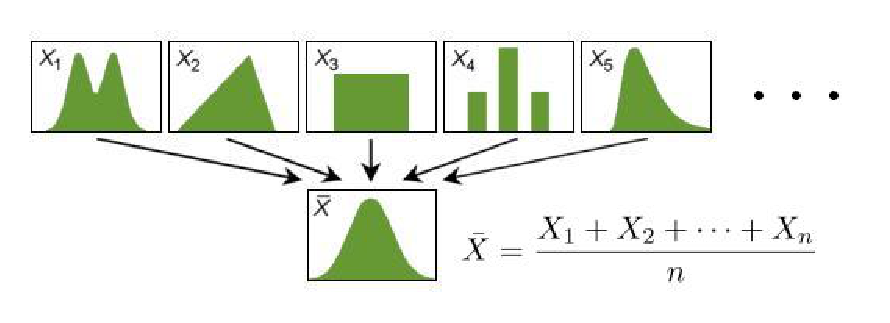
\includegraphics[width=0.7\textwidth]{normal/central_limit_theorem.eps}
\caption{中心极限定理}
\end{figure}

概率学家们进一步的研究结果更加令人惊讶,序列求和最终要导出正态分布的条件并不需
要这么苛刻,即便 $X_1,\cdots, X_n$ 并不独立,也不具有相同的概率分布形式,很多时
候他们求和的最终归宿仍然是正态分布。一切的纷繁芜杂都在神秘的正态曲线下被消解
,这不禁令人浮想联翩。中心极限定理恐怕是概率论中最具有宗教神秘色彩的定理,如果
有一位牧师拿着一本圣经向我证明上帝的存在,我是丝毫不会买账;可是如果他向我展示
中心极限定理并且声称那是神迹,我可能会有点犹豫,从而乐意倾听他的布道。如果我能
坐着时光机穿越到一个原始部落中,我也一定带上中心极限定理,并劝说部落的酋长把正
态分布作为他们的图腾。

中心极限定理虽然表述形式简洁,但是严格证明它却非常困难。中心极限定理就像一张大
蜘蛛网,棣莫弗和拉普拉斯编织了它的雏形,可是这张网上漏洞太多,一个多世纪来,数
学家们就像蜘蛛一样前赴后继,努力想把所有的漏洞都补上。在19世纪,泊松
(Sim\'{e}on Denis Poisson, 1781-1840)、狄利克莱(Gustav Lejeune Dirichlet,
1805-1859)、柯西(Augustin-Louis Cauchy, 1789-1857)、贝塞尔(Friedrich Bessel,
1784-1846)这些大蜘蛛都曾经试图对把这张网上的漏洞补上。从现代概率论的角度来看,
整个19世纪的经典概率理论并没有能输出一个一般意义下的严格证明。而最终把漏洞补上
的是来自俄罗斯的几位蜘蛛侠:切比雪夫(Pafnuty Chebyshev, 1821-1894)、马尔可夫(Andrey Andreyevich Markov,
1856-1922)和李雅普诺夫(Aleksandr Mikhailovich Lyapunov, 1857-1918)。

俄罗斯是一个具有优秀数学传统的民族,产生过几位顶尖的的数学家,在现代概率论的发展中,俄
罗斯的圣彼得堡学派可以算是顶了大半边天,而切比雪夫正是圣彼得堡数学学派的奠基人和领袖。
把中心极限定理证明中的漏洞补上的方案的雏形是从切比雪夫
1887年的工作开始的,切比雪夫提出了一个基于矩法的证明,矩法是概率分析中比较传统的方法,
使用的数学工具比较基础,不过切比雪夫这个证明也还存在一些漏洞。马尔可夫和李雅普诺夫都是切
比雪夫的学生,两人在中心极限定理的严格证明上展开了竞赛。马尔科夫在概率论里面可算是大名鼎鼎,
马尔科夫链是应用最为广泛的概率模型之一。马尔科夫和他的老师切比雪夫一样,他们在数学中的
研究风格都偏向于使用初等、简单易懂的数学工具来证明复杂艰深的定理。
马尔科夫沿着老师的基于矩法的思路在蜘蛛网上辛勤编织,在证明上做了很多的修补,但洞还是补得
不够严实。李雅普诺夫不像马尔可夫那样深受老师的影响,他沿着拉普拉斯当年提出的基
于特征函数的思路,于1901年给出了一个补洞的方法,切比雪夫对这个方法大加赞赏,李
雅普诺夫的证明被认为是第一个在一般条件下的严格证明;而马尔科夫也不甘示弱,在
1913年基于矩法也把洞给补严实了。

\begin{figure}[htbp]
\centering
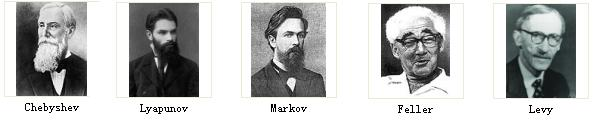
\includegraphics[width=1.0\textwidth]{normal/clt_proof.jpg}
\caption{华山论剑}
\end{figure}

20世纪初期到中期,中心极限定理的研究几乎吸引了所有的概率学家,这个定理俨然成为
了概率论的明珠,成为了各大概率论武林高手华山论剑的场所。不知道大家对中心极限定
理中的“中心”一词如何理解,许多人都认为“中心”这个词描述的是这个定理的行为:以
正态分布为中心。这个解释看起来确实合情合理,不过并不符合该定理被冠名的历史。事
实上,20世纪初概率学家大都称呼该定理为极限定理(Limit Theorem),由于该定理在概率
论中处于如此重要的中心位置,如此之多的概率学武林高手为它魂牵梦绕,于是数学家波
利亚于1920年在该定理前面冠以“中心”一词,由此后续人们都称之为中心极限定理。

数学家们总是极其严谨苛刻的,给定了一个条件下严格证明了中心极限定理,数学家们就开
始探寻中心极限定理成立的各种条件,询问这个条件是否充分必要条件,并且进一步追问
序列和在该条件下以什么样的速度收敛到正态分布。1922年林德伯格(Jarl Waldemar
Lindeberg, 1876-1932) 基于一个比较宽泛容易满足的条件,为中心极限定理提出了一个很
容易理解的初等证明,这个条件我们现在称之为林德伯格条件。然后概率学家费勒
(William Feller, 1906-1970) 和列维就开始追问:林德伯格条件是充分必要的吗?基于林
德伯格的工作, 费勒和列维都于 1935 年独立的得到了中心极限定理成立的充分必要条件
,这个条件可以用直观的非数学语言描述如下:

\begin{theorem}[中心极限定理充要条件]
假设独立随机变量序列 $X_i$ 的中值为0, 要使序列和 $\displaystyle S=\sum_{i=1}^n
X_i$ 的分布密度函数逼近正态分布,以下条件是充分必要的:
\begin{enumerate}
\item 如果 $X_i$相对于序列和$S$的散布(可以理解为标准差)是不可忽略的,则 $X_i$ 的分
      布必须接近正态分布;
\item 对于所有可忽略的 $X_i$, 取绝对值最大的那一项,这个绝对值相对于序列和
      也是可忽略的。
\end{enumerate}
\end{theorem}

事实上这个充分必要条件发现的优先权,费勒和列维之间还着实出现了一些争论,当然他
们俩都是独立的几乎在同一时间解决了这个问题。在列维证明这个充分必要条件的过程中
,列维发现了正态分布的一个有趣的性质。我们在数理统计中都学过,如果两个独立随机
变量 $X,Y$ 具有正态分布,则$S=X+Y$ 也具有正态分布;奇妙的是这个定理的逆定理也成
立:

\begin{theorem}[正态分布的血统]
如果 $X,Y$ 是独立的随机变量,且 $S=X+Y$ 是正态分布,那么 $X,Y$ 也是正态分布。
\end{theorem}

正态分布真是很奇妙,就像蚯蚓一样具有再生的性质,你把它一刀切两断,它生成两个正态
分布;或者说正态分布具有极其高贵的优良血统,正态分布的组成成分中只能包含正态分
布,而不可能含有其它杂质。

一流的数学家都是接近上帝的人,善于猜测上帝的意图。
1928 年 列维就猜到了这个定理,并在1935年使用这个定理对中心极限定理的充分必要条
件作了证明。有意思的是列维却无法证明正态分布的这个看上去极其简单的再生性质,
所以他的证明多少让人觉得有些瑕疵。不过列维的救星很快就降临了,1936 年
概率学家克拉美(Harald Cram\'{e}r, 1893-1985)证明列维的猜想完全正确。

中心极限定理成为了现代概率论中首屈一指的定理,事实上中心极限定理在现代概率论里
面已经不是指一个定理,而是指一系列相关的定理。统计学家们也基于该定理不断的完善
拉普拉斯提出的元误差理论,并据此解释为何世界上正态分布如此常见。而中心极限定理
同时成为了现代统计学中大样本理论的基础。

\subsection{进军近代统计学}

花开两朵,各表一枝。上面说了正态分布在概率论中的发展,现在来看看正态分布在数理
统计学中发展的故事。这个故事的领衔主演是凯特勒(Adolphe Quetelet, 1796-1874)和高
尔顿 (Francis Galton, 1822-1911)。
\begin{figure}[ht]
\centering
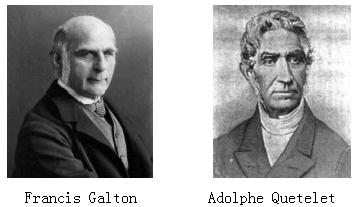
\includegraphics[width=0.5\textwidth]{normal/galton_quetelet.jpg}
\caption{凯特勒和高尔顿}
\end{figure}

由于高斯的工作,正态分布在误差分析中迅速确定了自己的地位。有了这么好的工具,我们
可能拍脑袋就认为,正态分布很快就被人们用来分析其它的数据,然而事实却出乎我们的
意料,正态分布进入社会领域和自然科学领域,可是经过一番周折的。

首先我要告诉大家一个事实:误差分析和统计学是风马牛不相及的两个学科;当然这个事
实存在的时间是19世纪初之前。统计学的产生最初是与“编制国情报告”有关,主要服务
于政府部门。统计学面对的是统计数据,是对多个不同对象的测量;而误差分析研究的是
观测数据,是对同一个对象的多次测量。观测数据和统计数据在当时被认为是两种不
同行为获取得到的数据,适用于观测数据的规律未必适用于统计数据。 19世纪的数据统计
分析处于一个很落后的状态,和概率论没有多少结合。概率论的产生主要和赌博相关,发
展过程中与误差分析紧密联系,而与当时的统计学交集非常小。将统计学与概率论真正结
合起来推动数理统计学发展的便是我们的统计学巨星凯特勒。

凯特勒这名字或许不如其它数学家那么响亮,估计很多人不熟悉,所以有必要介绍一下
。 凯特勒是比利时人,数学博士毕业,年轻的时候曾追随拉普拉斯学习过概率论。此人
学识渊博,涉猎广泛,脑门上的桂冠包括统计学家、数学家、天文学家、社会学家、国际
统计会议之父、近代统计学之父、数理统计学派创始人。 凯特勒 的最大的贡献就是将
法国的古典概率理论引入统计学,用纯数学的方法对社会现象进行研究。

1831年,凯特勒参与主持新建比利时统计总局的工作。他开始从事有关人口问题的统计学
研究。在这种研究中,凯特勒发现,以往被人们认为杂乱无章的、偶然性占统治地位的社会
现象,如同自然现象一样也具有一定的规律性。 凯特勒 搜集了大量关于人体生理测量
的数据,如体重、身高与胸围等,并使用概率统计方法来对数据进行数据分析。但是当时
的统计分析方法遭到了社会学家的质疑,社会学家们的反对意见主要在于:社会问题与科
学实验不同,其数据一般由观察得到,无法控制且经常不了解其异质因素,这样数据的同
质性连带其分析结果往往就有了问题,于是社会统计工作者就面临一个如何判断数据同质
性的问题。凯特勒大胆地提出:
{\bf 把一批数据是否能很好地拟合正态分布,作为判断该批数据是否同质的标准。}
\begin{figure}[H]
\centering
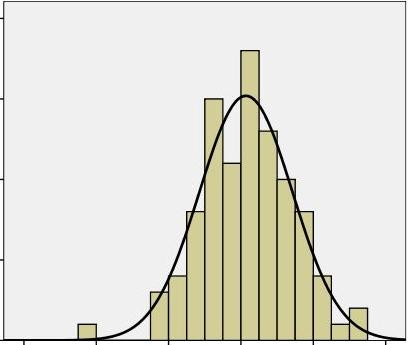
\includegraphics[width=0.35\textwidth]{normal/normal_fitness.jpg}
\caption{用正态分布拟合数据}
\end{figure}

凯特勒提出了一个使用正态曲线拟合数据的方法,并广泛的使用正态分布去拟合各种类
型的数据。由此, 凯特勒为正态分布的应用拓展了广阔的舞台。正态分布如同一把屠龙
刀,在凯特勒 的带领下,学者们挥舞着这把宝刀在各个领域披荆斩棘,攻陷了人口、领
土、政治、农业、工业、商业、道德等社会领域,并进一步攻占天文学、数学、物理学、
生物学、社会统计学及气象学等自然科学领域。

正态分布的下一个推动力来自生物学家高尔顿,当正态分布与生物学联姻时,近代统计学
迎来了一次大发展。高尔顿是生物统计学派的奠基人,他的表哥达尔文的巨著《物种起源
》问世以后,触动他用统计方法研究遗传进化问题。受凯特勒的启发,他对正态分布怀
有浓厚的兴趣,开始使用正态分布去拟合人的身高、胸围、以至考试成绩等各类数据,发
现正态分布拟合得非常好。他因此相信正态曲线是适用于无数情况的一般法则。

然而,对高尔顿而言,这个无处不在的正态性给他带来一些困惑。他考察了亲子两代的身
高数据,发现遵从同一的正态分布,遗传作为一个显著因素是如何发挥作用的?1877年,
高尔顿设计了一个叫高尔顿钉板(quincunx, 或者Galton board)的装置,模拟正态分布的
性质,用于解释遗传现象。

\begin{figure}[H]
\begin{center}
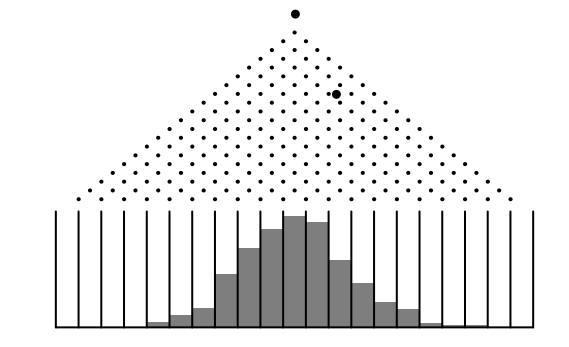
\includegraphics[width=0.5\textwidth]{normal/galton_quincunx.jpg}
\caption{高尔顿钉板}
\end{center}
\end{figure}

图中每一点表示钉在板上的一颗钉子,它们彼此的距离均相等。当小圆球向下降落过程中
,碰到钉子后皆以 1/2 的概率向左或向右滚下。如果有n排钉子,则各槽内最终球的个数
服从二项分布 $B(n,1/2)$, 当$n$ 较大的时候,接近正态分布。设想在此装置的中间某个
地方 AB 设一个挡板把小球截住,小球将在AB处聚成正态曲线形状,如果挡板上有许多阀
门,打开一些阀门,则在底部形成多个大小不一的正态分布,而最终的大正态分布正是这
些小正态分布的混合。

\begin{figure}[ht]
\centering
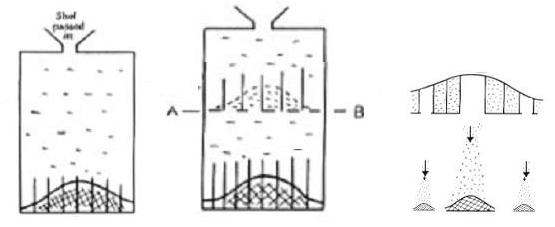
\includegraphics[width=0.6\textwidth]{normal/galton_quincunx3.jpg}
\caption{高尔顿钉板解释遗传现象}
\end{figure}

高尔顿利用这个装置创造性的把正态分布的性质用于解释遗传现象。他解释说身高受到显
著因素和其它较小因素的影响,每个因素的影响可以表达为一个正态分布。遗传作为一个
显著因素,类似图中底部大小不一的正态分布中的比较大的正态分布,而多个大小不一正
态分布累加之后其结果仍然得到一个正态分布。

网络上有人开发了一些好玩的程序用于模拟高尔顿钉板,我们可以动态的观察这些小球自上
而下滚动的时候,是如何形成正态分布的。一个使用 Java 开发的很漂亮的动态模拟可以在
如下网页中观察到:http://www.math.psu.edu/dlittle/java/probability/plinko/index.html。

\begin{figure}[ht]
\centering
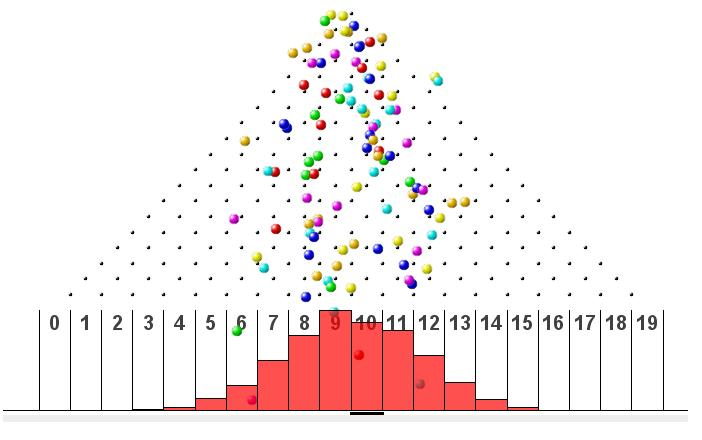
\includegraphics[width=0.8\textwidth]{normal/galton_quincunx5.jpg}
\caption{高尔顿钉板动态模拟程序}
\end{figure}

高尔顿在研究身高的遗传效应的时候,同时发现一个奇特的现象:高个子父母的子女,其
身高有低于其父母身高的趋势,而矮个子父母的子女,其身高有高于其父母的趋势,即有
“回归”到普通人平均身高去的趋势,这也是“回归”一词最早的含义。高尔顿用二维正
态分布去拟合父代和子代身高的数据,同时引进了回归直线、相关系数的概念,从而开创
了回归分析这门技术。

\begin{figure}[ht]
\centering
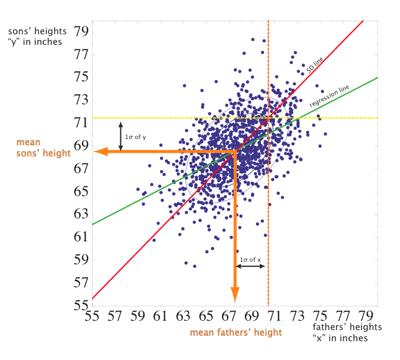
\includegraphics[width=0.5\textwidth]{normal/regression.jpg}
\caption{儿子与父亲的身高回归线}
\end{figure}

可以说,高尔顿是用统计方法研究生物学的第一人,他用实际行动开拓了凯特勒的思想
,为数理统计学的产生奠定了基础。无论是 凯特勒 还是高尔顿,他们的统计分析工作
都是以正态分布为中心的,在他们的影响下,正态分布获得了普遍认可和广泛应用,甚至
是被滥用,以至有些学者认为19世纪是正态分布在统计学中占统治地位的时代。

\subsection{数理统计三剑客}

最后,我们来到了20世纪,正态分布的命运如何呢?如果说19世纪是正态分布在统计学中
独领风骚的话,20世纪则是数理统计学蓬勃发展、百花齐放的时代。 1901年,高尔顿和他
的学生卡尔.皮尔逊(Karl Pearson, 1857-1936)、韦尔登(Walter Frank Raphael
Weldon, 1860-1906) 创办《生物计量 (Biometrika)》杂志,成为生物统计学派的一面旗帜
,引导了现代数理统计学的大发展。统计学的重心逐渐由欧洲大陆向英国转移,使英国在
以后几十年数理统计学发展的黄金时代充当了领头羊。

在20世纪以前,统计学所处理的数据一般都是大量的、自然采集的,所用的方法以拉普拉
斯中心极限定理为依据,总是归结到正态。到了19世纪末期,数据与正态拟合不好的情况
也日渐为人们所注意:进入20世纪之后,人工试验条件下所得数据的统计分析问题,逐渐
被人们所重视。由于试验数据量有限,那种依赖于近似正态分布的传统方法开始招受质疑
,这促使人们研究这种情况下如何能找到更加准确的统计方法。

\begin{figure}[ht]
\centering

\includegraphics[width=0.5\textwidth]{normal/non-normal.jpg}
\caption{非正态分布}
\end{figure}

在这个背景之下,统计学三大分布$\chi^2$分布、$t$分布、$F$分布逐步登上历史舞台。
这三大分布现在的理科本科生都很熟悉。在历史上,这三个分布和来自英国的现代数理
统计学的三大剑客有着密切的关系。

\begin{figure}[ht]
\centering
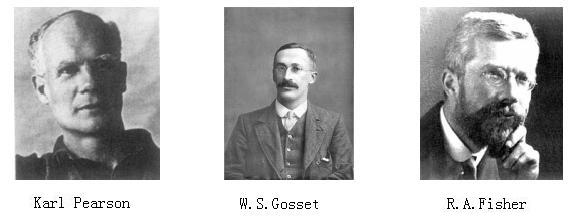
\includegraphics[width=0.9\textwidth]{normal/three-swords.jpg}
\caption{数理统计三剑客}
\end{figure}

第一位剑客就是卡尔.皮尔逊,手中的宝剑就是$\chi^2$分布。 $\chi^2$ 分布这把宝剑最
早的锻造者其实是物理学家麦克斯韦,他在推导空气分子的运动速度的分布的时候,发现
分子速度在三个坐标轴上的分量是正态分布,而分子运动速度的平方$v^2$ 符合自由度为3
的$\chi^2$分布。麦克斯韦虽然造出了这把宝剑,但是真正把它挥舞得得心应手、游刃有
余的是皮尔逊。在分布曲线和数据的拟合优度检验中,$\chi^2$分布可是一个利器,而皮
尔逊的这个工作被认为是假设检验的开山之作。皮尔逊继承了高尔顿的衣钵,统计功力深
厚,在19世纪末20世纪初很长的一段时间里,一直被数理统计武林人士尊为德高望重的第
一大剑客。

第二位剑客是戈塞特(William Sealy Gosset, 1876-1937),笔名是大家都熟悉的学生氏
(Student),而他手中的宝剑是 $t$ 分布。戈塞特是化学、数学双学位,依靠自己的化学
知识进酿酒厂工作,工作期间考虑酿酒配方实验中的统计学问题,追谁卡尔.皮尔逊学习了
一年的统计学,最终依靠自己的数学知识打造出了$t$分布这把利剑而青史留名。 1908年
,戈塞特提出了正态样本中样本均值和标准差的比值的分布,并给出了应用上极其重要的
第一个分布表。戈塞特在$t$ 分布的工作开创了小样本统计学的先河。

第三位剑客是费希尔(Ronald Aylmer Fisher, 1890-1962),手持$F$分布这把宝剑,在一
片荒芜中开拓出方差分析的肥沃土地。 $F$分布就是为了纪念费希尔而用他的名字首字母
命名的。费希尔剑法飘逸,在三位剑客中当属费希尔的天赋最高,各种兵器的使用都得心
应手。费希尔统计造诣极高,受高斯的启发,系统的创立了极大似然估计剑法,这套剑法
现在被尊为统计学参数估计中的第一剑法。

费希尔还未出道,皮尔逊已经是统计学的武林盟主了,两人岁数相差了33岁,而戈塞特介
于他们中间。三人在统计学擂台上难免切磋剑术。费希尔天赋极高,年少气盛;而皮尔逊
为人强势,占着自己武林盟主的地位,难免固执己见,以大欺小,费希尔着实受了皮尔逊
不少气。而戈塞特性格温和,经常在两位大侠之间调和。毕竟是长江后浪推前浪,一代新
人换旧人,在众多擂台比试中,费希尔都技高一筹,而最终取代了皮尔逊成为数理统计学
第一大剑客。

由于这三大剑客和统计三大分布的出现,正态分布在数理统计学中不再是一枝独秀,数理
统计的领地基本上是被这三大分布抢走了半壁江山。不过这对正态分布而言并非坏事,我
们细看这三大分布的数学细节: 假设独立随机变量 $X_i \sim N(0,1), Y_j \sim N(0,1)
(i=1\cdots n, j=1\cdots m)$,则满足三大分布的随机变量可以如下构造出来
\begin{enumerate}
\item $ \displaystyle \chi_n^2 = X_1^2 + \cdots + X_n^2$
\item $ \displaystyle  t = \frac{Y_1}{\sqrt{\frac{X_1^2 + \cdots + X_n^2}{n}}}$
\item $ \displaystyle  F = \frac{\frac{X_1^2 + \cdots + X_n^2}{n}}{\frac{Y_1^2 + \cdots + Y_m^2}{m}} $
\end{enumerate}

你看这三大分布哪一个不是正态分布的嫡系血脉,$\chi^2$、 $t$、$F$这三大分布最初都
是从正态分布切入进行研究的。所以正态分布在19世纪是武则天,进入20世纪就学了慈
禧太后,垂帘听政了。或者,换个角度说,一个好汉三个帮,正态分布如果是孤家寡人恐
怕也难以雄霸天下,有了统计学三大分布作为开国先锋为它开疆拓土,正态分布真正成为
傲世群雄的君王。

20世纪初,统计学这三大剑客成为了现代数理统计学的奠基人。以哥塞特为先驱,费希尔
为主将,掀起了小样本理论的革命,事实上提升了正态分布在统计学中的地位。在数理统
计学中,除了以正态分布为基础的小样本理论获得了空前的胜利,其它分布上都没有成功
的案例,这不能不让人对正态分布刮目相看。在随后的发展中,相关回归分析、多元分析
、方差分析、因子分析、布朗运动、高斯过程等等诸多概率统计分析方法陆续登上了历史舞台
,而这些和正态分布密切相关的方法,成为推动现代统计学飞速发展的一个强大动力。

\section{正态魅影}

\begin{quotation}
\it{Everyone believes in it: experimentalists believing that it is a
mathematical theorem, mathematicians believing that it is an empirical fact. \\
--- Henri Poincar\'{e}}
\end{quotation}

如果说,充斥着偶然性的世界是一个纷乱的世界,那么    正态分布为这个纷乱的世界建立
了一定的秩序,使得偶然性现象在数量上被计算和预测成为可能。杰恩斯在《概率论沉思
录》中提出了两个问题:
\begin{enumerate}
\item 为什么正态分布被如此广泛的使用?
\item 为什么正态分布在实践使用中非常的成功?
\end{enumerate}

\begin{figure}[!ht]
\centering
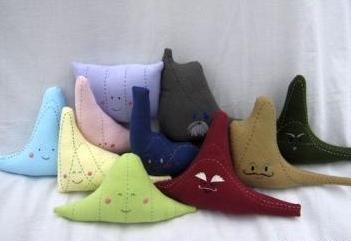
\includegraphics[width=0.5\textwidth]{normal/multi-normal-pillow.jpg}
\caption{无处不在的正态分布}
\end{figure}

杰恩斯指出,正态分布在实践中成功的被广泛应用,主要是因为正态分布在数学方面的具
有多种稳定性质,这些性质包括:
\begin{enumerate}
\item 两个正态分布密度的乘积还是正态分布
\item 两个正态分布密度的卷积还是正态分布,也就是两个独立正态分布随机变量的和还是服从正态分布
\item 正态分布$N(0, \sigma^2)$的傅立叶变换正规化为密度分布后还是正态分布
\item 中心极限定理保证了多个随机变量的求和效应将导致正态分布
\item 正态分布和其它具有相同均值、方差的概率分布相比,具有最大熵
\end{enumerate}

前三个性质说明了正态分布一旦形成,就容易保持该形态的稳定, 兰登对于正态分布的
推导也表明了,正态分布可以吞噬较小的干扰而继续保持形态稳定。后两个性质则说明,
其它的概率分布在各种的操作之下容易越来越靠近正态分布。正态分布具有最大熵的性质
,所以任何一个对指定概率分布的操作,如果该操作保持方差的大小,却减少已知的知识
,则该操作不可避免的增加概率分布的信息熵,这将导致概率分布向正态分布靠近。

正由于正态分布的多种稳定性质,使得它像一个黑洞一样处于一个中心位置,其它的概
率分布形式在各种操作之下都逐渐向正态分布靠拢,杰恩斯把它描述为概率分布中的重力现
象(gravitating phenomenon)。
\begin{figure}[htbp]
\centering
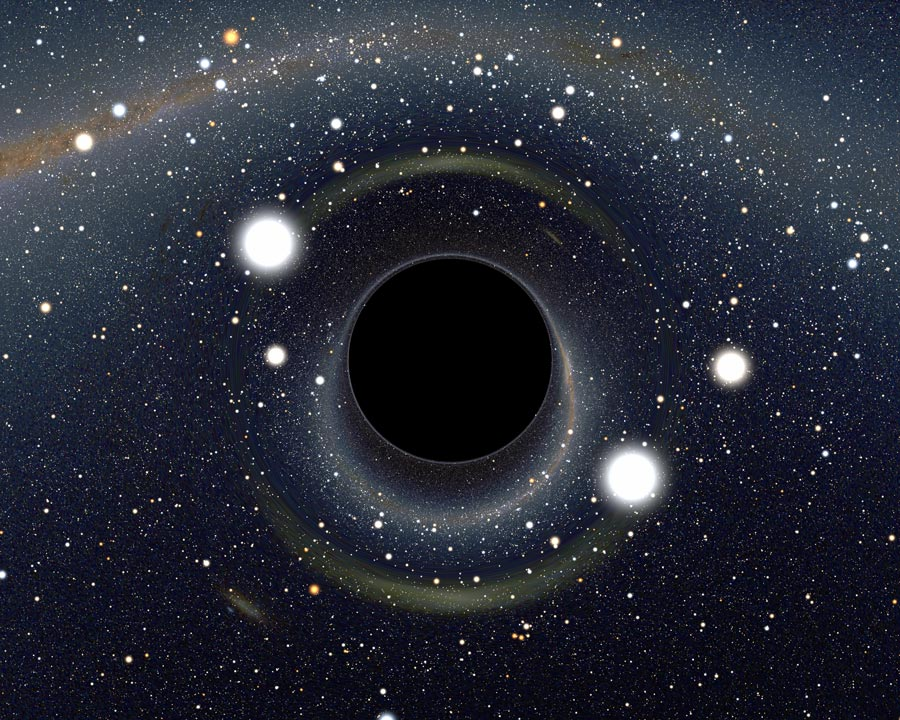
\includegraphics[width=0.5\textwidth]{normal/blackhole2.jpg}
\caption{正态黑洞}
\end{figure}

我们在实践中为何总是选择使用正态分布呢,正态分布在自然界中的频繁出现只是原因之
一,杰恩斯认为还有一个重要的原因是正态分布的最大熵性质。在很多时候我们其实没有
任何的知识知道数据的真实分布是什么, 但是一个分布的均值和方差往往是相对稳定的。
因此我们能从数据中获取到的比较好的知识就是均值和方差,除此之外没有其它更加有用
的信息量。因此按照最大熵的原理,我们应该在给定知识的限制下,选择熵最大的概率
分布,而这就恰好就是正态分布。即便数据的真实分布不是正态分布,由于我们对真实分布
一无所知,如果数据不能有效提供除了均值和方差之外的更多的知识,按照最大熵的原理
,正态分布就是这时候的最佳选择。

当然正态分布还有更多令人着迷的数学性质,我们可以欣赏一下:
\begin{itemize}
\item 二项分布 $B(n,p)$ 在 $n$很大逼近正态分布 $N(np, np(1-p))$
\item 泊松分布 $Poisson(\lambda)$ 在 $\lambda$ 较大时逼近正态分布 $N(\lambda,\lambda)$
\item $\chi^2_{(n)}$在 $n$很大的时候逼近正态分布 $N(n,2n)$
\item $t$分布在 $n$ 很大时逼近标准正态分布 $N(0,1)$
\item 正态分布的共轭分布还是正态分布
\item 几乎所有的极大似然估计在样本量$n$增大的时候都趋近于正态分布
\item 克拉美分解定理(之前介绍过):如果 $X,Y$ 是独立的随机变量,且 $S=X+Y$ 是正
      态分布,那么 $X,Y$ 也是正态分布
\item 如果 $X,Y$ 独立且满足正态分布$N(\mu, \sigma^2)$, 那么 $X+Y$, $X-Y$ 独立且
      同分布,而正态分布是唯一满足这一性质的概率分布
\item 对于两个正态分布$X,Y$, 如果$X,Y$ 不相关则意味着$X,Y$独立,而正态分布是唯
      一满足这一性质的概率分布
\end{itemize}

\section{大道至简,大美天成}

%\begin{verse}
%\emph{To see a world in a grain of sand \\
%And a heaven in a wild flower, \\
%Hold infinity in the palm of your hand \\
%And eternity in an hour. \\}
%\end{verse}

$$\overline{X} = \frac{X_1 + X_2 + \cdots + X_n}{n} $$
算术平均,极其简单而朴素的一个式子,被人们使用了千百年,在其身后隐藏着一个美丽
的世界,而正态分布正是掌管这个美丽世界的女神。正态分布的发现与应用的最初历史,
就是数学家们孜孜不倦的从概率论和统计学角度对算术平均不断深入研究的历史。中心极
限定理在 1773年棣莫弗的偶然邂逅的时候,它只是一粒普通的沙子,两百多年来吸引了众
多的数学家,这个浑金璞玉的定理不断的被概率学家们精雕细琢,逐渐的发展成为现代概
率论的璀璨明珠。而在统计学的误差分析之中,高斯窥视了造物主对算术平均的厚爱,也
发现了正态分布的美丽身影。殊途同归,那是偶然中的必然。一沙一世界,一花一天国,
算术平均或许只是一粒沙子,正态分布或许只是一朵花,它们却包含了一个广阔而美丽的
世界,几百年来以无穷的魅力吸引着科学家和数学家们。


\begin{figure}[ht]
\centering

\includegraphics[width=0.7\textwidth]{normal/world-grain.jpg}
\end{figure}

高尔顿他对正态分布非常的推崇与赞美,1886 年他在人类学研究所的就职演讲中说过一段
著名的话:“我几乎不曾见过像误差呈正态分布这么美妙而激发人们无穷想象的宇宙秩序
。如果古希腊人知道这条曲线,想必会给予人格化乃至神格化。它以一种宁静无形的方式
在最野性的混乱中实施严厉的统治。暴民越多,无政府状态越显现,它就统治得越完美。
他是无理性世界中的最高法律。当我们从混沌中抽取大量的样本,并按大小加以排列整理
时,那么总是有一个始料不及的美妙规律潜伏在其中。”

概率学家卡克在他的自述传记《机遇之谜》(Enigmas of chance: An autobiography)
中描述他与正态分布的渊源:“我接触到正态
分布之后马上被他深深的吸引,我感到难以相信,这个来自经验直方图和赌博游戏的规律
,居然会成为我们日常生活数学的一部分。”另一位概率学家 Michel
Lo\'{e}ve(1907-1979) 说:“如果我们要抽取列维的概率中心思想,那我们可以这样说,
自从 1919 年以后,列维研究的主题曲就是正态分布,他一而再再而三的以她为出发点,
并且坚决的又回到她......  他是带着随机时钟沿着随机过程的样本路径作旅行的人。”
美国国家标准局的顾问 W. J. Youden 用如下一段排列为正态曲线形状的文字给予正态分
布极高的评价,意思是说:误差的正态分布规律在人类的经验中具有“鹤立鸡群”的地位
,它在物理、社会科学、医学、农业、工程等诸多领域都充当了研究的指南,在实验和
观测数据的解读中是不可或缺的工具。

\begin{figure}[ht]
\centering
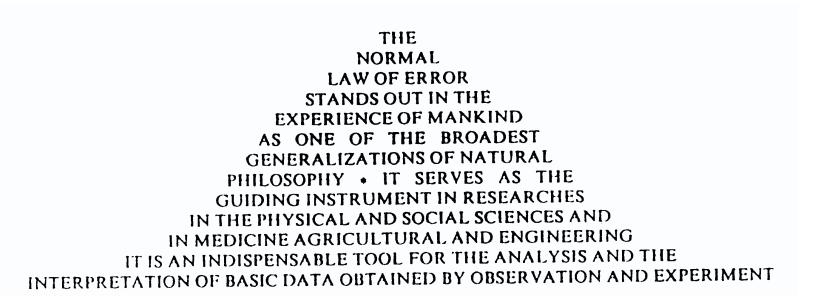
\includegraphics[width=1.0\textwidth]{normal/youden-normal-curve.jpg}
\caption{正态误差态分布律}
\end{figure}

几乎所有的人都或多或少的接触数学,虽然各自的目的不同,对数学的感觉也不同。工程
师、科学家们使用数学是因为他简洁而实用,数学家们研究数学是因为它的美丽动人。像
正态分布这样,既吸引着无数的工程师、科学家,在实践中被如此广泛的应用,又令众多
的数学家为之魂牵梦绕的数学存在,在数学的世界里也并不多见。我在读研究生的时候,
经常逛北大未名BBS 的数学板,有一个叫 ukim 的著名 ID 在精华区里面留下了一个介绍
数学家八卦的系列《Heroes in My Heart》,写得非常的精彩,这些故事在喜欢数学的人
群中也流传广泛。最后一个八卦是关于菲尔兹奖得主法国数学家托姆(Ren\'{e} Thom)的,
它曾经令无数人感动,我也借用来作为我对正态分布的八卦的结语:

\begin{quotation}
\kaishu{在一次采访当中,作为数学家的托姆同两位古人类学家讨论问题。谈到远古的人们为什么
要保存火种时,一个人类学家说,因为保存火种可以取暖御寒;另外一个人类学家说,因
为保存火种可以烧出鲜美的肉食。而托姆说,因为夜幕来临之际,火光摇曳妩媚,灿烂
多姿,是最美最美的......}
\end{quotation}

\begin{figure}[htb]
\centering
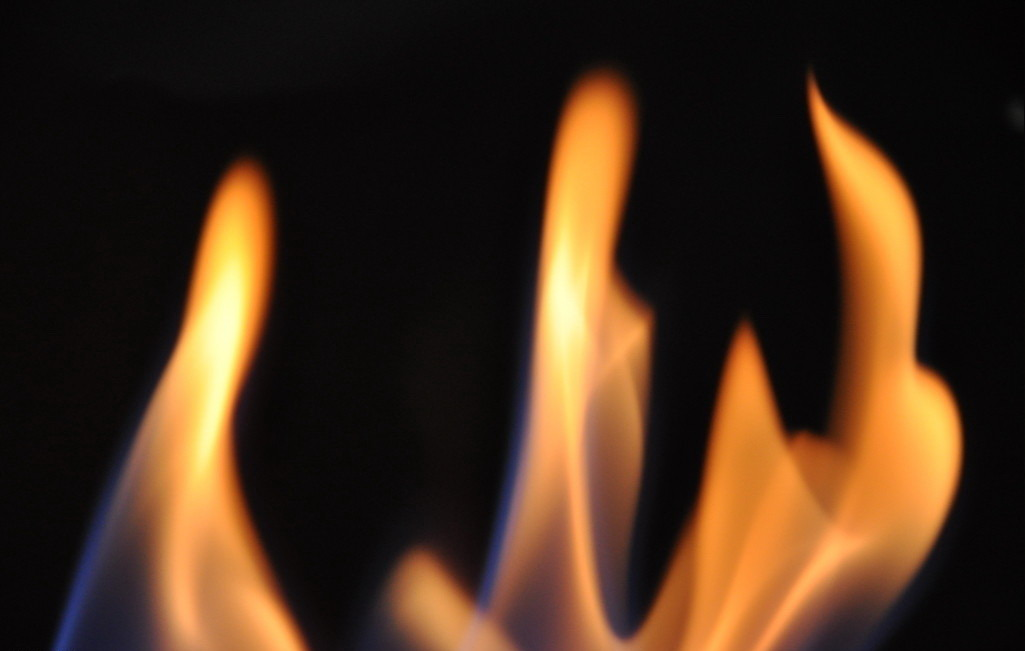
\includegraphics[width=0.6\textwidth]{normal/fire.jpg}
\end{figure}

\newpage
\section{推荐阅读}

\begin{verse}
\emph{All knowledge is, in the final analysis, history.  \\
All sciences are, in the abstract, mathematics.  \\
All methods of acquiring knowledge are, essentially, through \mbox{statistics.} \\}

\kaishu{在终极的分析中,一切知识都是历史;\\
在抽象的意义下,一切科学都是数学; \\
在理性的基础上,所有的判断都是统计学。\\}

\emph{--- C. R. Rao}
\end{verse}

本人并非统计学专业人士,只是凭个人兴趣做一点知识的传播。对统计学历史知识的介绍
,专业性和系统性都不是我的目的,我更在乎的是趣味性,因为没有趣味就不会有传播。
如果读完这段历史会让你觉得正态分布更加亲切,不再那么遥不可及,那我的目的达到了
。如果正态分布是一滴水,我愿大家都能看到它折射出的七彩虹。

本文所使用的大多是二手资料,有些历史细节并没有经过严格的考证,对于历史资料一定
程度上按照个人喜好做了取舍,本文主要基于如下的资料写成,对于历史细节感兴趣的,
推荐阅读。

\begin{itemize}
\item 陈希孺, 数理统计学简史,湖南教育出版社,2000
\item 蔡聰明,誤差論與最小平方法,数学传播 21(3):3-13,1994
\item 吴江霞,正态分布进入统计学的历史演化,2008
\item E.T. Jaynes, Probability Theory: The Logic of Science,Cambridge University Press,2003
\item Saul Stahl, The Evolution of the Normal Distribution, Mathematics Magazine, 1996
\item Kiseon Kim, Georgy Shevlyakov, Why Gaussianity, IEEE Signal Processing Magazine, 2008
\item Stephen M. Stigler, The History of Statistics: The Measurement of Uncertainty before, Belknap Press of Harvard University Press, 1990
\item L. Le Cam, The Central Limit Theorem Around 1935, Statistical Science 1(1):78-91, 1986
\item Hans Fischer, A History of the Central Limit Theorem: From Classical to Modern Probability Theory, Springer, 2010
\end{itemize}
